% Talk of Volume Preserving Mean Curvature Motion
\documentclass[10pt]{beamer}
\usepackage{settings-my-talk}
\includeonlyframes{ slide/frame1,%
                    slide/frame2,%
                    slide/frame3,%
                   }

%
%
% General Informations
\title{Uno schema Semi-Lagrangiano per il moto per curvatura media che
  preserva il volume}
\author{Michele Cipolla \\
\texttt{cipmiky@gmail.com}}
\institute[Dip. Matematica]{Univeristà la Sapienza di Roma}
\date{23 Luglio 2014}
%\logo{
\includegraphics[width=0.05\textwidth]{logoSapienzaHalf}}
%
%
% Customize Theme
%\definecolor{sapC}{rgb}{0.53,0.15,0.15}
%\usetheme{Antibes}
%\usetheme{Berlin}
%\usetheme{Berkeley}
\usetheme{CambridgeUS}
%\setbeamercolor*{structure}{fg=sapC}
%\setbeamerfont{size=\Large, series=\bfseries,
%  family=\rmfamily}
\setbeamertemplate{headline}
{%
  \begin{beamercolorbox}{section in head/foot}
    \vskip2pt \insertnavigation{\paperwidth}\vskip2pt
   \end{beamercolorbox}
}
\setbeamertemplate{footline}
{%
  \begin{beamercolorbox}{section in head/foot}
    \vskip2pt \insertpagenumber\vskip2pt
   \end{beamercolorbox}
}
%
%
%
\begin{document}
%
%
% Title page
\begin{frame}
\titlepage
\end{frame}
%
%
% Table of contents
\section*{Outline}
\begin{frame}{Outline}
\tableofcontents
\end{frame}
%
%
% Central Frame
\begin{frame}
  \frametitle{Motivazioni}
  \begin{columns}[t]
    \begin{column}{4cm}
       \begin{block}{Deterioramento delle immagini}
         Processi di acquisizione di immagini traminte scanner 3D o di
         trasferimento delle stesse, possono deteriorale generando del
         \alert{rumore}. 
       \end{block}
     \end{column}
     \begin{column}[T]{6cm}
      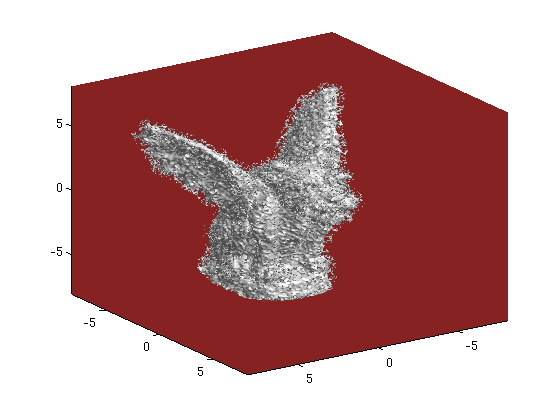
\includegraphics[width=1.0\textwidth]{noise/imnoise/mcm/gargolye/garg149i-0-00}
     \end{column}
  \end{columns}
\end{frame}

\section{Modello}
\begin{frame}{Moto per curvatura media}
     \begin{block}{}
       \begin{itemize}
       \item $S$ superfice regolare in $\mathbb{R}^3$
       \item $\mathcal{S}(p,t)$ parametrizzazione di $S$
       \item $\mathcal{N}(x,t)$ vettore unitario normale regolare
       \item $\mathcal{H}=-\Div(\mathcal{N})\mathcal{N}$ vettore curvatura media
       \end{itemize}
     \end{block}
     \begin{block}{}
       $(x_1,x_2,x_3)\in S_t$ evolve seconde il sitema parabolico
       \[
       \left\{
       \begin{aligned}
         &\mathcal{S}_t(p,t)=-\Div(\mathcal{N})\mathcal{N}\text{ $t>0$} \\
         &\mathcal{S}(0)=S
       \end{aligned}
       \right.
       \]
     \end{block}
\end{frame}

\begin{frame}{Collasso in un punto}
  \begin{columns}[c]
    \begin{column}{6cm}
      \begin{block}{Superfici convesse}
       Superfici convesse  evolvono in un
       punto in un tempo finito.
       \end{block}
      \begin{exampleblock}{Evoluzione della Sfera}
        Una famiglia di sfere $\mathcal{S}(p,t)=S^2(R(t))$ con
        $R(0)=R_0$, si evolve secondo
        \[
        \begin{aligned}
          \overset{\displaystyle.}{R}(t) &= -\frac{2}{R(t)},\,
          R(0)=R_0,\Rightarrow\\
          R(t)&=\sqrt{R_0^2-4t}\Rightarrow, \\
          R(t)&=0 \Longleftrightarrow t=\frac{R_0^2}{4}<\infty 
        \end{aligned}
        \]
      \end{exampleblock}
    \end{column}
    \begin{column}[c]{4cm}
       \begin{center}
     \only<2->{\animategraphics[autoplay,loop,width=1.0\textwidth,height=0.45\textheight]{0.8}{smooth/mcm/sphere/sphere50-}{0}{4}}
     \end{center}
    \end{column}
    \end{columns}
\end{frame}

\begin{frame}{Possibili cambiamenti topologici e singolarità}
  \begin{columns}[c]
    \begin{column}{5cm}
      \begin{block}{Superfici non convesse}
       Superfici non convesse possono subire cambiamenti topologici
       generando delle singolartà. 
       \end{block}
      \begin{exampleblock}{Evoluzione del Manubrio}
        Il manubrio può essere considerato come due sfere di equal
        raggio connesse da un cilindro. A causa del collasso del
        cilindro in una linea, il manubrio si spezza in due sfere
        disconnesse.
      \end{exampleblock}
    \end{column}
    \begin{column}[c]{5cm}
       \begin{center}
     \only<2->{\animategraphics[autoplay,loop,width=1.0\textwidth,height=0.45\textheight]{0.8}{smooth/mcm/dumbbell/dumbb100-}{0}{5}}
     \end{center}
    \end{column}
    \end{columns}
\end{frame}


\begin{frame}{Flusso \emph{volume preserving}}
  \begin{columns}[T]
    \begin{column}{6cm}
      \begin{block}{Processo di nomalizzazione}
        Cambiamo la scala temporale
        \begin{itemize}
        \item $\mathcal{\tilde{S}(\tau)}=\psi(t)\mathcal{S}(t)$ 
        \item $\psi^2(t)=\frac{\partial\tau}{\partial t}$
        \end{itemize}
         in modo tale che \alert{$Volume_{\tau}\equiv 0$}, ottenendo   
         \begin{itemize}
         \item $\mathcal{\tilde{S}}_t=\left(\mathcal{\tilde{H}}-\frac{\rho\iint\mathcal{\tilde{H}}d\mu}{3V_0}\right)\mathcal{N}$
         \item $\rho =-<\mathcal{\tilde{S}},\mathcal{N}>$
         \end{itemize}
      \end{block}
    \end{column}
    \begin{column}[T]{4cm}
      \begin{exampleblock}{Evoluzione della sfera}
        \begin{itemize}
        \item $\tau(t)=\int_0^t\frac{T}{T-\tilde{t}}d\tilde{t}$ con
          $T=\frac{R_0^2}{4}$ tempo di 
          collasso
        \item $\tilde{V}=\psi^3(t)V$
        \item $\tilde{V}=\left(\frac{T}{T-t}\right)^{\frac{3}{2}}V$
        \item $V=\frac{4}{3}\pi(R_0^2-4t)^{\frac{3}{2}}$
        \item $\tilde{V}=\frac{4}{3}\pi R_0^3=V_0$
        \end{itemize}
      \end{exampleblock}
    \end{column}
  \end{columns}
\end{frame}

\section{Formulazione level-set}
\begin{frame}{MCM \emph{volume preserving} in forma level-set}
  \begin{block}{Superfici come insiemi di livello}
    La superfice regolare $S$ è rappresentata come il livello $0$ di
    una funzione ausiliaria $u(x)\in C^{\infty}(\Omega)$
    \begin{itemize}
      \item $S=\{x\in\Omega | u(x)=0\}$ e $Du(x)\neq 0$ in $S$
      \item $\mathcal{N}=-\frac{Du(x)}{|Du(x)|}$ vettore normale
        regolare
    \end{itemize}
  \end{block}
  \begin{block}{Equazione in forma level-set}
    La famiglia di curve regolare $S_t$
    \begin{itemize}
      \item $S_t=\{x\in\Omega | u(x,t)=0\}$ con $u(x,t)$ definita in
        $\Omega\times I$ e tale che $Du(x,t)\neq 0$ in $S_t$
      \item $x_0\in S_{t_0}$, $x(t)\in S_t$ curva regolare in
        $I_{\delta}(t_0)$ tale che $x(t_0)=x_0$
      \item $u(x(t),t)=0$ derivando \alert{velocità normale}$=\frac{u_t(x_0,t_0)}{|Du(x_0,t_0)|}$
    \end{itemize}
  \end{block}
\end{frame}

\begin{frame}{Flusso VPMCM}
  In forma level-set abbiamo
    \[
      (\text{VPMCM})\,u_t=|Du(x,t)|\Div\left(\frac{Du(x,t)}{|Du(x,t)|}\right)-\frac{\iint\Div\left(\frac{Du(x,t)}{|Du(x,t)|}\right)d\mu}{3V_0}x^tDu(x,t). 
      \]
  \begin{block}{Parte MCM e termine di traporto} 
    \begin{itemize}
    \item parte MCM 
      \[
      |Du(x,t)|\Div\left(\frac{Du(x,t)}{|Du(x,t)|}\right)=tr(P(Du)D^2u)
      \]
      \item $P(Du)=I-\frac{b\otimes }{|b|^2}\,b\in\mathbb{R}^3$
        matrice di proezione sul piano ortogonale a $b$
      \item parte di trasporto, non locale. 
        \[
        \mathcal{I}(\mathcal{H}(u),t)=\frac{\iint\Div\left(\frac{Du(x,t)}{|Du(x,t)|}\right)d\mu}{3V_0}
        \]
     \end{itemize}
  \end{block}
\end{frame}

\begin{frame}{Vantaggi forma level-set}
 \begin{block}{Vantaggi}
   \begin{itemize}
     \item Forma level-set scritta in un sistema di coodinate fisso
     \item I cambiamenti topologici non sono un problema. Topologia di
       $u$ è fissa.
     \item L'emergere di discontinuità, per alcune velocità è ben
       posto nella teoria viscosa
   \end{itemize}
 \end{block}

\end{frame}



\begin{frame}{Problema ben posto nella teoria viscosa}
     \begin{block}{Classe dell'equazione}
       La nostra equazione VPMCM \alert{$u_t+F(x,u,Du,D^2u)=0$}
       rappresenta un PDE parabolico non lineare singolare nei punti in cui
       il grandiente di $u$ si annulla ed è ben posto nella teoria
       delle solulzioni viscose. $F$ del tipo
       \begin{itemize}
         \item $F:\Omega\times\mathbb{R}\times\mathbb{R}^n\times
           S(n)\to\mathbb{R}$, $S(n)$ matrici simmetriche e
           $\Omega\subset\mathbb{R}^n$
         \item $u_t+F(x,r,p,X)=0$
       \end{itemize}
     \end{block}
\end{frame}

\begin{frame}{Soluzioni di viscosità}
  \begin{definizione}
    Sia $\Omega$ aperto di $\mathbb{R}^n$ e $T>0$. Sia $F$ continua in
    $W=\overline{\Omega}\times
    [0,T]\times\mathbb{R}\times\mathbb{R}^n\times S(n)$ a valori in
    $\mathbb{R}$. Sia $\mathcal{O}$ aperto in $\Omega\times(0,T)$.
    \begin{itemize}
      \item Una funzione $u:\mathcal{O}\to\mathbb{R}$ semicontinua
        superiormente è una \alert{sotto
          soluzione viscosa} di 
        \[
        u_t+F(x,t,u,Du,D^2u)=0
        \]
        in $\mathcal{O}$ se per ogni $\phi\in C^2(\mathcal{O})$ e
        $\hat{z}=(\hat{x},\hat{t})\in\mathcal{O}$ tale che $(u-\phi)$ ha
        massimo in $\hat{z}$ allora
        \[
        \phi_t(\hat{z})+F(\hat{z},\phi(\hat{z}),D\phi(\hat{z}),D^2\phi(\hat{z}))\leq 0
        \]
        \item $u$ semicontinua inferiomente e una \alert{sopra
          soluzione viscosa}  in $\mathcal{O}$ se per ogni coppia
          $\phi$ e $\hat{z}$ tale che $(u-\phi)$ ha min in $\hat{z}$
          vale che
          \[
          \phi_t(\hat{z})+F(\hat{z},\phi(\hat{z}),D\phi(\hat{z}),D^2\phi(\hat{z}))\geq 0
          \]
        \end{itemize}
  \end{definizione}
\end{frame}

\begin{frame}{Proprietà di confronto}
  \begin{osservazione}
    Nel caso $F$ non sia continua, la definizione di solulzione
    viscosa continua a valere per l'inviluppo semicontinuo di
    $F$. Ricordiamo che data $h$ definita in $L\subset\mathbb{R}^n$
    \begin{itemize}
    \item  invluppo semicontinuo inferiore $h_*(x)=\lim_{r\to
      0}\inf\{h(y); y\in B_r(x)\cap L\}$ con $x\in\overline{L}$
    \item inviluppo semicontinuo superiore $h^*(x)=\lim_{r\to
      0}\sup\{h(y);y\in B_r(x)\cap L\}$ con $x\in\overline{L}$
    \end{itemize}
  \end{osservazione}
  \begin{block}{Propietà di confronto}
    Se $u$ è una sotto soluzione in $Q=\Omega\times[0,T)$ e
      $v$ una sopra  soluzione sempre in $Q$,  allora $u\leq
      v$ in $\mathcal{O}$ se $u\leq v$ sulla frontiera prabolica 
    \[
    \partial_pQ=\Omega\times\{0\}\cup\partial\Omega\times[0,T).
    \]
  \end{block}
\end{frame}

\begin{frame}{Esistenza e confronto in MCM e VPMCM}
  \begin{block}{Problema risolto}
    Nel caso MCM il flusso $F(p,X)=-tr(P(p)X)$ verifica
    \begin{enumerate}
    \item \alert{propria}: $F(x,r,p,X)\leq F(x,s,p,X)$ per $r\leq
      s$ e $\forall\,p\in\mathbb{R}^n$,$X\in S(n)$
    \item \alert{ellittica degenere}: $F(x,r,p,X)\leq
      F(x,r,p,Y)$ per $X\geq Y$
    \item \alert{geometrica}: $F(x,\lambda p,\lambda X+\sigma
      p\otimes p)=\lambda F(x,p,X)$, $\lambda >0,\sigma\in\mathbb{R}$
    %  \item $-\infty<F_*(x,0,O)=F^*(x,0,O)<\infty$
    \end{enumerate}
    sotto queste propietà valgono risultati di esistenza e confronto.
  \end{block}
  \begin{block}{Non abbiamo risultati definitivi}
    Nel caso VPMCM $F(x,u,p,X)=-tr(P(p)X)+b(u)x^tp$. In generale
    $b(u)$ non è costante quindi per esempio non è
    \alert{propria} è neanche \alert{giometrica}, sopravvive solo la
    proprietà di \alert{degenere ellitticità}; per cui  non possiamo
    utilizzare i risultati precedenti. Risultati definitivi su
    questi tipi di equaizioni ancora non ci sono.
  \end{block}
\end{frame}

%
%
% Reference 
\begin{frame}{Referenze}
\begin{thebibliography}{Goldbach, 1742}
\bibitem{Goldbach1742}[Goldbach, 1742]
  Christian Goldbach
  \newblock A open problem
  \newblock \emph{Letter to Leonhard Eulero}, 1742.

\bibitem{Goldbach1742}[Goldbach, 1742]
  Christian Goldbach
  \newblock A open problem
  \newblock \emph{Letter to Leonhard Eulero}, 1742.
\end{thebibliography}
\end{frame}
%
%
%
\end{document}


